\section{Word Embeddings \label{ssec: word embeddings}}

    \begin{figure}
        \centering
        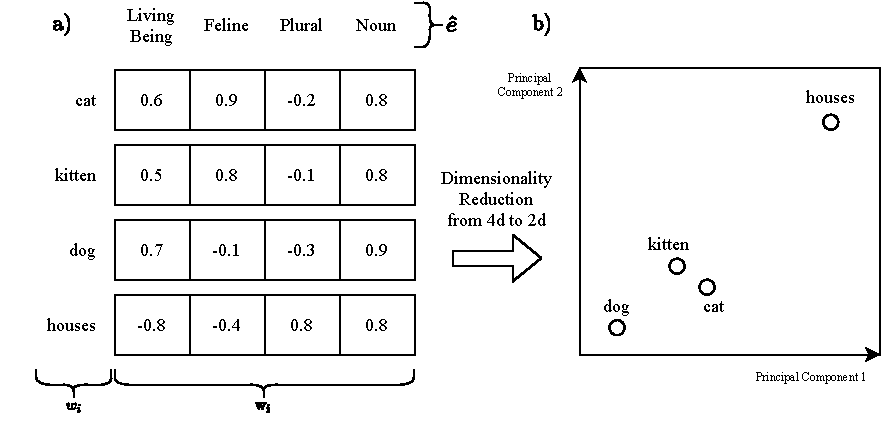
\includegraphics[width=0.9\textwidth]{embeddings.pdf}
        \caption{a) A schematic example of word \glspl{embedding} that represents each word in basis $\hat{e}$. In real-world embeddings, $\hat{e}$ is determined by the computer and has no human-understandable meaning. It also has much higher dimensionality. b) A graphical representation of the embedded words.}
        \label{fig:word embedding}
    \end{figure}

    For humans, (a large part of) learning a language is learning the mapping of words to their meanings such as ``dog" $\rightarrow$ pet with fur that makes ``woof" sound; ``table" $\rightarrow$ stable surface standing on legs etc. If a computer is to interpret textual information, we need to provide it with an analogous mapping. This is accomplished using word embeddings.
    Word \glspl{embedding} $\mathbf{w_i}$ are high-dimensional ($\approx 300$ dimensions) vectors of real numbers aiming to represent the semantic meaning of a word $w_i$. Fig. \ref{fig:word embedding} gives a simple example of such \glspl{embedding}. $\mathbf{w_i}$ are created by using large corpora of texts, (such as all Wikipedia articles, or a crawl through the entire internet) and using the context of words $w_i$ to learn their representation $\mathbf{w_i}$ in an unsupervised way. The basis for this is the assumption that similar words appear in similar contexts\cite{word2vec}.
    %Word \glspl{embedding} are at the heart of many \gls{nlp} applications and many pre-trained word \glspl{embedding} are available.
    The most prominent \glspl{embedding} are Google's, word2vec\cite{word2vec} and Stanford university's \gls{glove}\cite{glove} \glspl{embedding}. The lesser known \textit{ConceptNet Numberbatch} \glspl{embedding}\cite{conceptnet} build upon (and improve) both \gls{glove} and word2vec (see Sec. \ref{ssec: Numberbatch}).

    \subsection{GloVe \label{ssec: Glove}}
        \gls{glove}\cite{glove} (short for Global Vectors) is a mapping
        \[ \hat{f}(w_i) \rightarrow \mathbf{w_i}\]
        from words to \gls{embedding} vectors. It is trained on very large corpora such as Wikipedia or the entire internet. First, the co-occurence matrix $C_{ij}$ is created:

        \begin{equation}
        C_{ij} = \text{\# Co-occurences between words $i$ and $j$},
        \end{equation}

        where a co-occurence of two words means that they are featured within the same document, e.g. the same Wikipedia article or the same website. If there are $N_w$ words in the corpus, $C_{ij}$ is a $N_w \times N_w$ matrix, measuring the co-occurence between every word $w_i$ with every other word $w_j$.
        %For \gls{glove}, $N_w = \num{1.9e6}$ when trained on Wikipedia, $N_w = \num{2.2e6}$ when trained on a crawl of the entire internet.
        $C_{ij}$ is sparse, (meaning most entries are 0) as most words do not appear in the same context as most other words. By then performing dimensionality reduction (e.g. \gls{lda}) on $C_{ij}$, a dense representation of much lower dimensionality is obtained for every word. This representation is the word \gls{embedding}. For \gls{glove}, \glspl{embedding} are by default 300-dimensional\cite{glove}.

        Word2vec is trained in a similar way, though what counts as a co-occurence and how the dimensionality is reduced is slightly different\cite{word2vec}.

    \subsection{ConceptNet Numberbatch \label{ssec: Numberbatch}}

        ConceptNet is a open source semantic network that represents words (and short sequences of words commonly seen together) as nodes and the relationships between them as edges. An example is shown in Fig. \ref{fig: conceptnet}.
           \begin{figure}[h]
                \centering
                 \captionsetup{format=hang}
                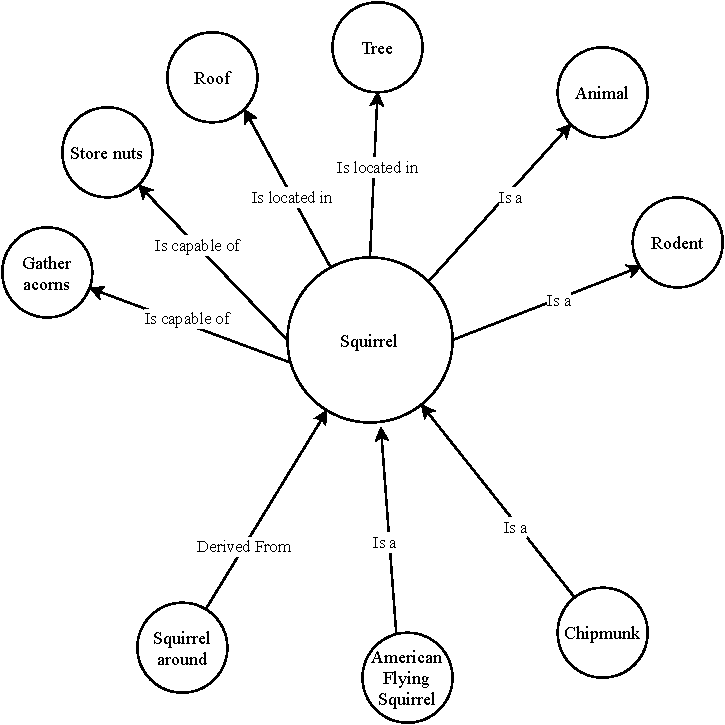
\includegraphics[width=0.7\textwidth]{conceptnet.pdf}
                \caption{Some of the connections of the word ``squirrel" in conceptNet. \label{fig: conceptnet}}
            \end{figure}

        By combining the ConceptNet network with other word \glspl{embedding} such as word2vec and \gls{glove} using a process called \textit{retrofitting}, a new, improved set of word \glspl{embedding}, the \textit{\gls{numberbatch}}, is created.

        \subsubsection{Retrofitting}
            Retrofitting uses a set of \glspl{embedding} $\mathbf{w_i}$, such as \gls{glove} or word2vec (Sec. \ref{ssec: Glove}) to infer new \glspl{embedding} $\Tilde{\mathbf{w_i}}$ that are both close to the original \glspl{embedding} and also close to their neighbours in the ConceptNet graph, by minimising the objective function
            \begin{equation}
                \Psi(W)=\sum_{i=1}^{N}\left[\alpha_{i}\left\|\mathbf{w}_{i}-\Tilde{\mathbf{w}}_{i}\right\|^{2}+\sum_{(i, j) \in E} \beta_{i j}\left\|\mathbf{w}_{i}-\mathbf{w}_{j}\right\|^{2}\right],
            \end{equation}
            where the sum is over all words included within the union of all words contained in ConceptNet with all words contained in the original \glspl{embedding}, $W$ is the set of all word \glspl{embedding} $\mathbf{w_i} \in W$, $E$ is the set of all edges within the ConceptNet graph, $\beta_{ij}$ is the weight of the edge between words $w_i$ and $w_j$ in the ConceptNet graph, and $\alpha_i$ are weights determining how important the previous \glspl{embedding} are compared to the edges within ConceptNet. How exactly $\alpha_i$ is determined is not explained within the original paper, but when a word is found within ConceptNet, that was not found within the \glspl{embedding}, $\alpha_i = 0$, allowing for a further expansion of the vocabulary.\cite{speer2017conceptnet}

        \subsubsection{Superior Performance}
            By combining word2vec, \gls{glove} and ConceptNet, the \gls{numberbatch} achieves superior performance in many word \gls{embedding} benchmarks\cite{speer2017conceptnet, conceptnetPerformance}.

        %\subsubsection{Mini Version}
            %As a convenience, the \gls{numberbatch} \glspl{embedding} are available as both more accurate 32-bit floating point numbers and as less accurate 8-bit integers. The 8-bit integer version allows for significantly smaller files (mini $\approx$ 50MB, full \glspl{embedding} $\approx$ 5GB) and loading times. We use the mini versions due to limited resources.

    \subsection{Similarity \label{ssec: cosine similarity}}
        The defining feature of word \glspl{embedding} is that semantically similar words have similar vectors. We can thus quantify the similarity $\eta_{ij}$ between two words $w_i, w_j$ as the cosine similarity of their \glspl{embedding}
        \begin{equation}
            \eta_{ij} = \text{cosine}(\mathbf{w_i}, \mathbf{w_j}) = \frac{\mathbf{w_i} \cdot \mathbf{w_j}}{|\mathbf{w_i}| |\mathbf{w_j}|}.
            \label{eq: cosine similarity}
        \end{equation}
        We use this notion of similarity heavily in this work.

    \subsection{Sentence Embeddings \label{ssec: utterance embeddings}}

    In the same way that words can be embedded based on a pre-trained set of \glspl{embedding}, sentences can be embedded also. Training the \glspl{embedding} doesn't work in the same way as for words (otherwise every sentence would have to be contained within the corpus for an \gls{embedding} to exist), but the concept is the same. A sentence is represented as a vector in a high-dimensional vector space. This allows a similarity between sentences to be computed as the cosine similarity (see Sec. \ref{ssec: cosine similarity}, Eq. \ref{eq: cosine similarity}). Examples include Google's universal sentence encoder\cite{GoogleEncoder} and Facebook's InferSent\cite{infersent}.

    \subsection{Limitations}
        \begin{figure}[ht]
            \centering
            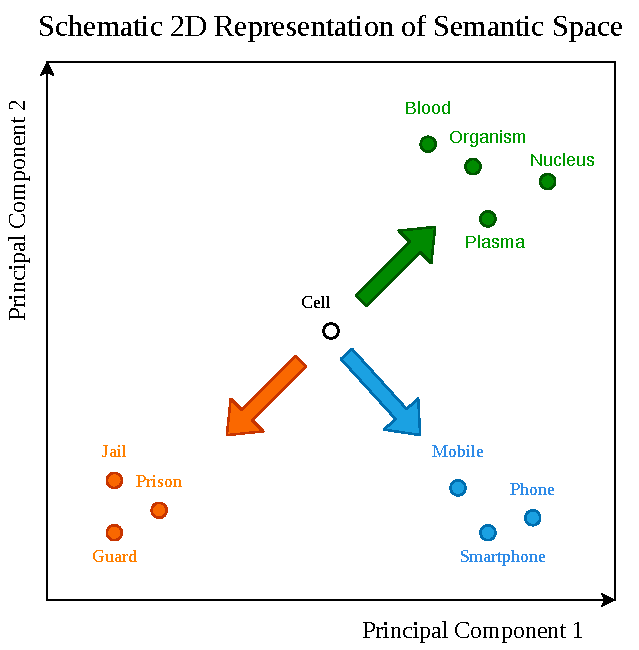
\includegraphics{ambiguous_embedding.pdf}
            \caption{Due to appearing frequently in contexts relating to biology, phones and prison, the word \gls{embedding} for the ambiguous word ``cell" is attracted to all three contexts in semantic space. The final \gls{embedding} lies somewhere in between the contexts and is a poor representation for all three meanings of ``cell".}
            \label{fig:ambiguous_embedding}
        \end{figure}

        Word \glspl{embedding} suffer from some limitations, the most significant of which is the problem of word-sense disambiguation, which occurs because words may have multiple meanings but only one \gls{embedding}. In the sentence
        \begin{align*}
            &\textit{``He went to the prison cell with his cell phone to extract blood cell samples}\\
            & \textit{from the inmates."}
        \end{align*}
        the word \textit{cell} appears 3 times and has a different meaning every time, but it has only one word \gls{embedding}. Because the method of \gls{embedding} is incapable of disambiguating the different meanings of the words, the word \gls{embedding} is poor: In the semantic vector space of word \glspl{embedding}, \textit{cell} will be attracted to words within its ``biology context", but also within its ``phone" context and within its ``prison" context, leading to a final \gls{embedding} somewhere in the middle, making it ineffective within all three contexts. The newest types of word \glspl{embedding}, such as BERT\cite{devlin2018bert} or ELMo\cite{peters2018elmo} address this problem by taking whole sentences as inputs and use the context of adjacent words to compute disambiguated word \glspl{embedding}.
